\section{Auswertung}
Das für die Auswertung der angefertigten Bilder und der Bestimmung der Interferenzmaxima verwendete Programm ist das Paket \textit{Fiji} der open-source-Anwendung \textit{ImageJ} \cite{Fiji}.

\subsection{Eichung des Magnetfeldes}
Zu Beginn des Auswertung soll das Magnetfeld des Elektromagneten geeicht werden. Hierzu werden die Strom-Magnetfeld-Paare für das ansteigende und das abfallende Magnetfeld aus Tabelle \ref{tab:eichen} grafisch aufgetragen.
Durch eine lineare Ausgleichsrechnung der Form
\begin{equation}
  B(I)=aI+b
\end{equation}
soll ein möglichst exaktes Bestimmen des über den Strom $I$ eingestellen Magnetfeldes $B$ erreicht werden.
Zu sehen ist dieser Zusammenhang in Abbildung \ref{abb:eichung}.
Als Parameter der Ausgleichsrechnung ergeben sich
\begin{align*}
  a = \SI{183,3 \pm 7,9}{\milli\tesla\per\ampere},\\
    b = \SI{-36,0 \pm 27,8}{\milli\tesla}\;.
\end{align*}

\begin{table}[H]
  \centering
  \caption{Messwerte der Magnetfeldstärke $B$ in Abhängigkeit der Stromstärke $I$ des verwendeten Elektromagneten jeweils bei ansteigenden und abfallenden Feldern.}
  \label{tab:eichen}
  \begin{tabular}{c|cc}
    \toprule
    {$I \:/\: \si{\ampere}$} & {$B_\text{steigend} \:/\: \si{\milli\tesla}$} & {$B_\text{fallend} \:/\: \si{\milli\tesla}$} \\
    \midrule
  0.0    &     5,5  &    6,3  \\
  0.5    &    111,8  &   105,3  \\
  1.0    &   155,5  &  163,7  \\
  1.6    &   242,4  &  244,1  \\
  2.0    &   318,2  &  310,3  \\
  2.5    &   390,0  &  406,9  \\
  3.0    &   469,9  &  474,7  \\
  3.5    &   550,7  &  554,9  \\
  4.0    &   629,2  &  642,8  \\
  4.6    &   734,7  &  746,6  \\
  5.1    &   880,9  &  879,2  \\
  5.5    &   1042,0  &  1015,4  \\
  6.0    &   1150,5  &  1150,5  \\
  \end{tabular}
\end{table}

\begin{figure}
  \centering
  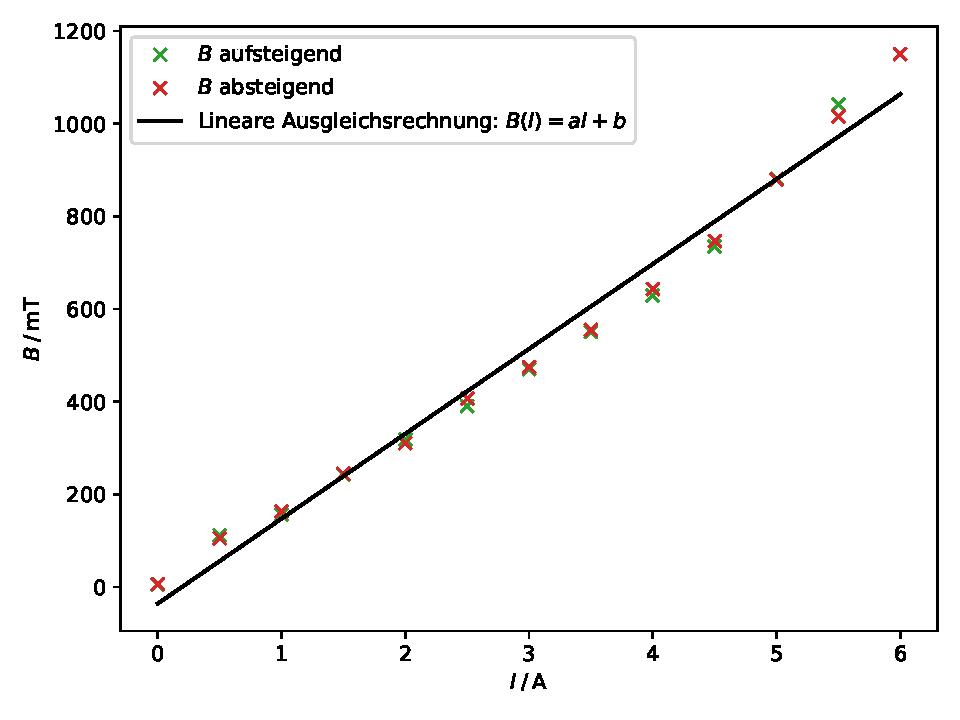
\includegraphics[width=0.7\textwidth]{plots/eichung.pdf}
  \caption{Das mit einer Hall-Sonde gemessene Magnetfeld $B$ in Abhängigkeit des eingestellten Stroms $I$ für ein Auf- und ein Absteigen. Ebenso eine lineare Ausgleichsrechnung zur Bestimmung des Wertepaarzusammenhangs.}
  \label{abb:eichung}
\end{figure}

\subsection{Messung des Landé-Faktors}
Im Folgenden sollen nun die Breiten der Interferenzstreifen ohne angelegtes Magnetfeldes $\deltaup$ und unter Einfluss eines angelegten Magnetfeldes $\Deltaup$ bestimmt werden.
Für die Wellenlängendifferenzen ergibt sich unter Verwendung der in Abschnitt \ref{sec:dispersion} bestimmten $\Deltaup \lambda$:
\begin{equation}
  \deltaup \lambda = \frac{1}{2}\frac{\deltaup s}{\Deltaup s}\Deltaup \lambda\,.
  \label{eq:difflambda}
\end{equation}
Die Energiedifferenz aufgrund eines angelegten Magnetfeldes ergibt sich zu
\begin{equation}
  |\Deltaup E| = |\Deltaup m| g \mu_B B\,.
\end{equation}
Für die Energie lässt sich $E=\frac{\hbar c}{\lambda}$ einsetzen und nach $\lambda$ ableiten.
Über Umformen des für $\deltaup \lambda$ eingesetzten Zusammenhangs \eqref{eq:difflambda} nach dem Landé-Faktor ergibt sich für die erlaubten Übergänge mit $|\Deltaup m|=1$
\begin{equation}
  g=\frac{\hbar c \delta \lambda}{\lambda^2 \mu_B B}\,.
\end{equation}
Mittels des Pakets \textit{Fiji} werden nun die aufgenommenen Fotographien auf ihren Farbkontrast hin ausgewertet.
Hierüber lassen sich die Abstände $\Deltaup$ und $\deltaup$ über die Funktion "Find Maxima" bestimmen.

\subsection{Vermessung der \texorpdfstring{$\sigma$}{sigma}-Komponente der roten Linie}

\subsection{Vermessung der \texorpdfstring{$\sigma$}{sigma}-Komponente der blauen Linie}

\subsection{Vermessung der \texorpdfstring{$\pi$}{pi}-Komponente der roten Linie}
